\section{Preparation}\label{sec:prep}
Before the data can be further processed and used, some simple preparation
must be done to normalise the data.
This section discusses the transformative steps and the end representation that
the program will work with from the initial state until classification.

\subsection{Resampling}
All recordings are normalised to the same format properties, since the source
material varies greately from sample to sample.

Variations include:
\begin{itemize}[noitemsep]
  \item Audio channels;
  \item Bit depth;
  \item Sample rate;
  \item Length.
\end{itemize}

If a recording is found to have more than a single channel, all but the left
channel are discarded.
Section~\ref{sec:reflections} reflects on wheter this is the best approach.

Sample rate reductions are made to reduce the memory and processing demands of
analysing all 231231 minutes of audio.
Our image recognition approach holds greater importance to the general shape
of individual vocalisations in spectrograms, rather than high time-frequency
details.
Because of this, the sample rate reduction is found to have no significant
reductions in classification quality.

The recording length is left unaltered.

The ffmpeg program is used to convert all source material to 22050 Hz 16-bit
WAV files.
We have written a shell script to make this procedure fully automatic, executable
when new recordings have been sourced.


\subsection{Spectrogram Representation}
A spectrogram is a visualisation of a sound as energy in the frequency spectrum
in function of time.
This allows us to intuitively visualise the shape of a sound in a 2d image.
Figure~\ref{fig:sgram_pcm} shows how the spectrogram representation retains
amplitude information from a waveform, while exposing the frequency composition
of the waveform.

\begin{figure}[!htb]
  \centering
  \begin{subfigure}[b]{1.0\textwidth}
    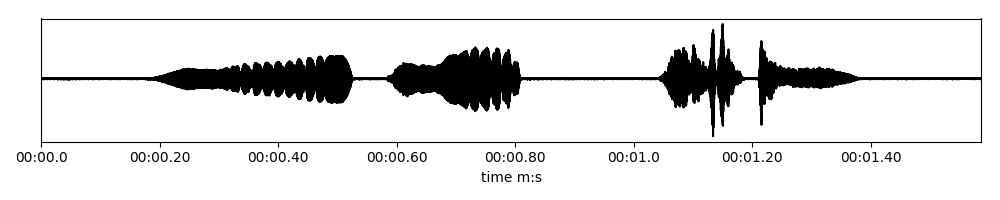
\includegraphics[width=1.0\textwidth]{pcm}
    \caption{}
  \end{subfigure}
  \begin{subfigure}[b]{1.0\textwidth}
    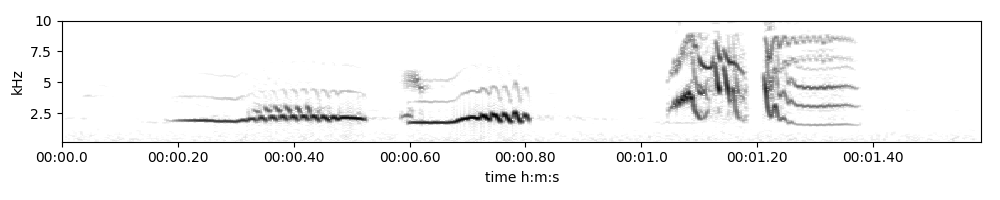
\includegraphics[width=1.0\textwidth]{sgram}
    \caption{}
  \end{subfigure}
  \caption{Waveform (a) and corresponding spectrogram (b) of a bird 1 recording}
  \label{fig:sgram_pcm}
\end{figure}

Our image recognition approach makes use of this spectrographic representation
of the field recordings.

Spectrogram construction is performed for all recordings.
Each recording is processed sequentially and immediately stored on disk.
The audio is first loaded as raw pulse-code modulation (Appendix~\ref{app:pcm}).
The Fast fourier transform (FFT) method is then used to generate a spectrogram
from the PCM (see Appendix~\ref{app:sgram} for details on constructing
spectrograms using FFTs).
Modern hardware handles FFT computations very well, making this stage very quick.
The Matplotlib |specgram| function is used to generate spectrograms.

The following parameters are used during spectrogram construction:
\begin{itemize}[noitemsep]
  \item \textbf{NFFT: 512}.
    NFFT defines the number of PCM data points used in each chunk.
  \item \textbf{Window: Hann window of 512 points.}
    Windowing is used to merge overlapping chunks.
  \item \textbf{Overlap: 75\%}.
    Overlap defines the number of points overlapping between chunks.
\end{itemize}

Spectrograms are converted to monochrome to simplify operations in the stages
to follow.
This does not reduce the information present in the spectrogram.

Frequencies above 10000Hz and below 100Hz are removed from the spectrograms as
these do not contain signals belonging to any bird species \textbf{(cite)}.
